\documentclass[../report.tex]{subfiles}
 
\begin{document}
\onehalfspacing

\newpage
\sektion{1}{Verified Boot}

\subsection{Security Promises}

The main purpose of Chrome OS's verified boot is to provide relative security to the end user without sacrificing usability or functionality. 
In its mission statement, verified boot is designed against an ``opportunistic hacker''~\cite{vboot-design-doc}.
This means that Vboot protects against simple vectors of attack that are relatively quick to exploit.
These types of attacks include but are not limited to faking Google's server to provide false firmware updates, installing a malicious kernel driver, or disabling the Vboot process to read user secrets stored in hardware.
Vboot accomplishes its goals by ensuring that all executed code during the boot process (from power on to user login) originates from Google's platform and is unmodified. 

Vboot does not make any promises to the safety of the system once the kernel is running and the user has control. 
The attack surface of the kernel and userspace is much larger, and security holes are found in user programs (such as a web browser) on a daily basis.
Vboot can assure the user that on every reboot, the system will either start in a clean, untampered state, or it will warn the user and provide steps for full recovery.

Verified Boot is designed in a way such that it only depends on a minimum set of secure hardware components for its guarantees.
As Chrome OS is an open source project, this allows the OS to be adapted to a number of normal laptops, without needing a specialized ChromeBook.

\subsection{Code Organization}

Like almost all modern operating systems, Chrome OS is written in C.
Like Linux, Chrome OS is maintained using Git for version control. 
Git is a diff-based, non-centralized version control system that makes it easy for programmers to share code, rollback changes, and maintain separate branches of the same codebase~\cite{git}.
Google has built a tool called ``repo'' that is used on top of git~\cite{repo}. 
Repo is a tool to manipulate multiple code repositories. 
It's primary benefit is that it allows a company to specify how multiple git repositories should be installed and placed within a given file-system.
This is both helpful and necessary as Chrome OS consists of over one thousand different external and internal repositories. 

Coreboot, vboot\_reference, depthcharge, are the repositories used for the firmware boot process, and they are explained below. 

\subsubsection{Coreboot}

Coreboot is a fully Open-Sourced alternative to traditional BIOS implementations.~\cite{coreboot}
It is lightweight and is configured to implement the full standard of the Unified Extensible Firmware Interface (UEFI).
Google has chosen Coreboot because of its small code footprint, full extensibility, and the fact that it is available freely as an Open Source project.

The Coreboot code is mostly responsible for doing very early initialization code on the main CPU\@. 
% This includes things like setting up the GPIO pins, enabling hardware interrupts, setting up a large stack in RAM, and providing driver callbacks to the payload that it will eventually call.
Coreboot is setup so that once a baseline level of initialization is complete, it passes control to another section of code called a ``payload'' ~\cite{coreboot-payload}.
This payload is responsible for initializing the more specialized drivers, and the concept of a payload means that Google can keep support more hardware without altering the Coreboot source code.
The payload that Coreboot calls to further initialize the Chromebook is Depthcharge.
% Init done in src/mainboard/google/{link}/romstage.c

% TODO: Who is responsible for loading the Flashmap into MMIO? 

\subsubsection{DepthCharge}

Depthcharge contains the minimum number of drivers necessary for the virtual boot to work successfully~\cite{depthcharge-codebase}. 
The important drivers include the TPM, I2C, the EC, SPI and SPI Flash, and the display~\cite{depthcharge-slides}.
Once the drivers are initialized successfully, Depthcharge creates the necessary structures for Vboot and then passes control into the Vboot library.

\subsubsection{Vboot\_reference}

The vboot\_reference repo contains all of the control and algorithms for the vboot process~\cite{vboot-codebase}.
The repo is designed such that it does not rely on any knowledge about the chipset or the firmware that is running. 
If a function requires usage of a driver or something that is board specific, it will make a callback into Depthcharge which will provide the relevant information.
%TODO: should I list relevant files and directories here?

% \subsection{Board Specifics}
%
%Chromebooks are created by many different vendors and can have very different hardware and capabilities.


\subsection{Verified Boot Stages}

Google has engineered Chrome OS to make all possible assurances that it boots into a correct and untampered state. 
The boot process of a laptop is very complex and will include very different code across different laptops and hardware versions. 
In order to accomplish this security in a reasonable fashion and have Secure Boot be extensible for current and future chipsets, Google has split the process into three main sections as seen in Figure~\ref{fig:fw_process}.
These sections are referred to as Read-Only Firmware (RO FW), Read-Write Firmware (RW FW), and Kernel.

\begin{figure}
\begin{subfigure}{.4\textwidth}
  \centering
  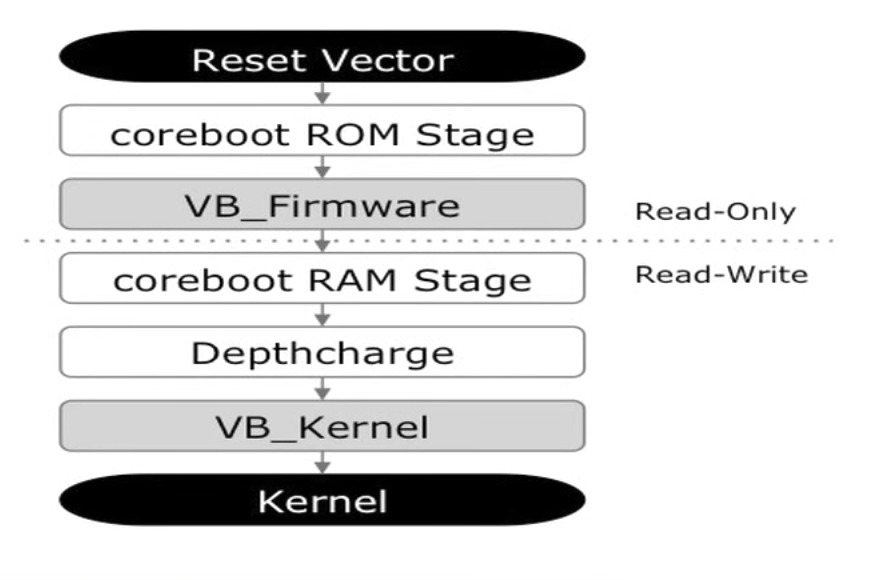
\includegraphics[width=1.0\linewidth]{vboot_stages_overview.png}
\end{subfigure}%
\begin{subfigure}{.60\textwidth}
  \centering
  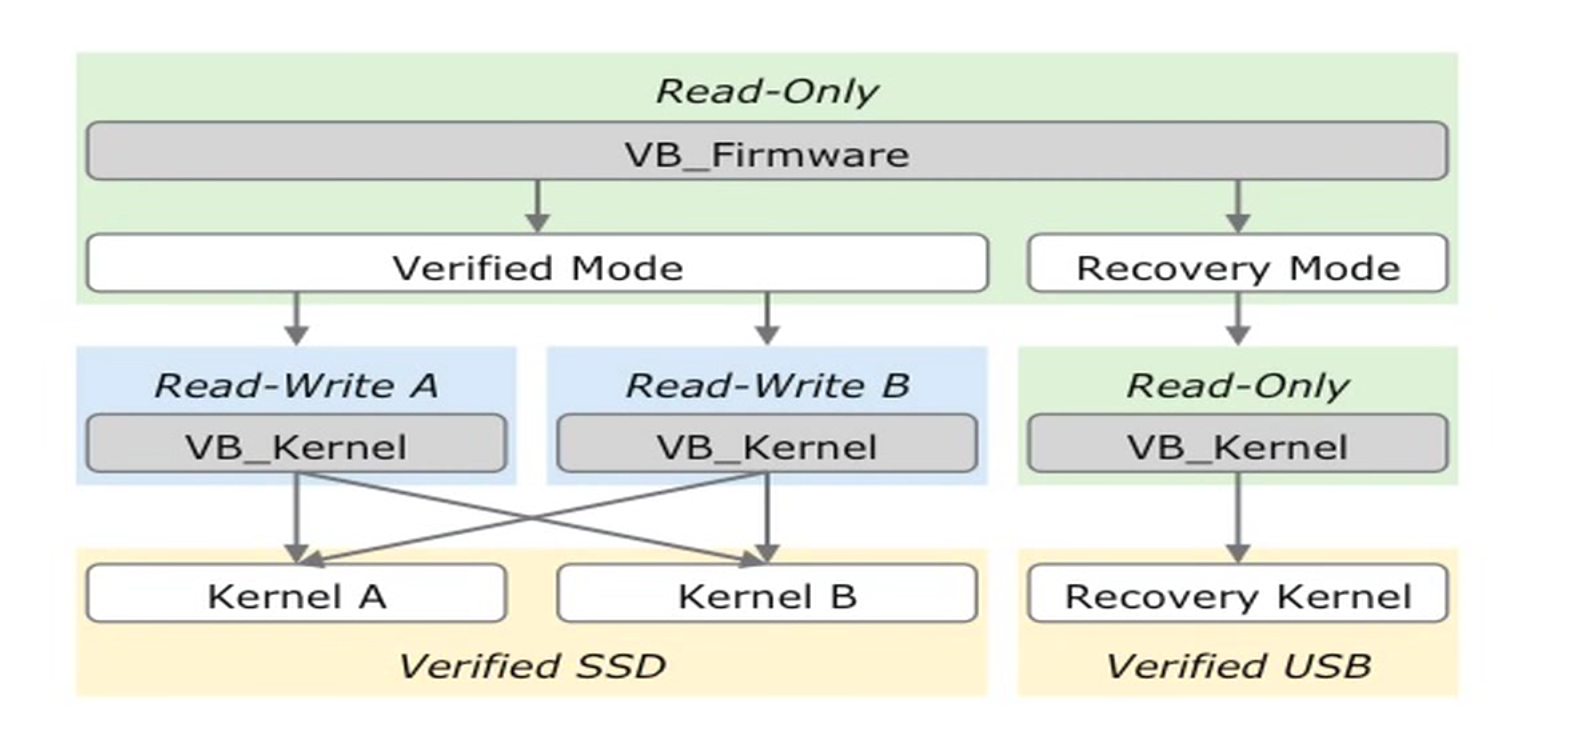
\includegraphics[width=1.0\linewidth]{vboot_stages_AB_recovery.png}
\end{subfigure}
\caption{Verified Boot is separated into hierarchical stages for clarity and security}
\label{fig:vboot_stages_overview}
\end{figure}

% TODO: Move this to a Security section
% Root of Trust
%In security all algorithms are based on a ``Root of Trust''.
%A Root of Trust is the lowest part of a security algorithm, it is the information that must be trusted as there is no way to verify it.
%The root of trust for Vboot is the Read-Only Firmware Section (RO FW).
%This section is stored in the Flash section of memory of the chip, in a section
%that is set as Read Only by a removable screw located within the laptop.

The RO Firmware runs first and is only responsible for the drivers that are necessary to drive the Vboot process. 
It's primary responsibility is finding the RW Firmware and verifying its correctness. 
It is also responsible for handing the main control of Vboot, such as the transitions between Developer Mode, Safe Mode, and Recovery Mode.
The RO Firmware also takes care of locking parts of the TPM for the rest of the boot process.

% RW FW
The RO Firmware passes control to the RW Firmware once it garauntees its security.
The RW FW initializes the rest of the hardware on the chip and begins verification of the kernel.
The main responsibility of RW Firmware for Vboot is initializing the disk drivers and loading the kernel into RAM.
RW Firmware is also responsible for updating and attesting the state of the EC.

\subsection{Boot Modes}

Vboot has an extra surface of attack from a normal verified boot because of the possibility of a transition from a normal, protected state to an unprotected state and back again.
The unprotected state is labeled ``Developer Mode'' and it can be set by the user of the device after logging in~\cite{developer-mode}. 
% TODO: verify that flag is in Flash memory
Developer Mode can be turned on either by a physical switch on the device or by setting a flag high in Flash memory.
% TODO: verify that RO checks dev for hash
When Developer Mode is enabled, the RO and RW Firmware no longer checks that the next stage is signed by the previous stage's key combination.
Google allows this mode so that hobbyists and enthusiasts can manipulate the hardware to its full extent.
With Developer Mode enabled, people have been able to load full Linux Operating Systems to the Chromebook after writing their own firmware.

Developer Mode is a security hole by nature, so various precautions are in place around its usage. 
First, a physical presence is required to fully complete the developer mode transition. 
This means that a person must sit at the computer once it has been rebooted and press a certain key combination (Control + D) when the developer mode screen appears.
The physical presence exists such that developer mode cannot be enabled through an off-site software attack without the user's knowledge.
The developer mode screen is referred to internally as the ``Scary Screen'', and its purpose is also to prevent users from being tricked into enabling developer mode by an external phishing party.

Once Developer Mode has been enabled, the TPM is wiped as it stores secure user data (such as passwords) and it's safety cannot be guaranteed in an insecure system.
The partition on disk that stores user data is also wiped in this transition, as it again contains encrypted user secrets that would be vulnerable to an open system.

These precautions are also taken on the transition back from Developer Mode to Safe Mode. 
In order to put the machine back into Safe Mode, Recovery Mode must be activated first, and the system must be restored by a Recovery USB\@.
The path to use the Recovery USB is stored in RO Firmware, and it will reset and clear the TPM as well as reformat the contents on disk before supplying new firmware and kernel partitions. 

\subsection{Data Structures}

Here is a list of the data structures used in Vboot~\cite{vboot-data-structures}.
These data structures are populated at the beginning of the Vboot process by being read in from either SPI Flash (Firmware Data) or the main hard drive (Kernel Data).
Through this section I will start at the highest hierarchical level of data structure then explain the structures that are contained within.

\subsubsection{Firmware/Kernel Image}

\begin{figure}
\begin{subfigure}{.5\textwidth}
  \centering
  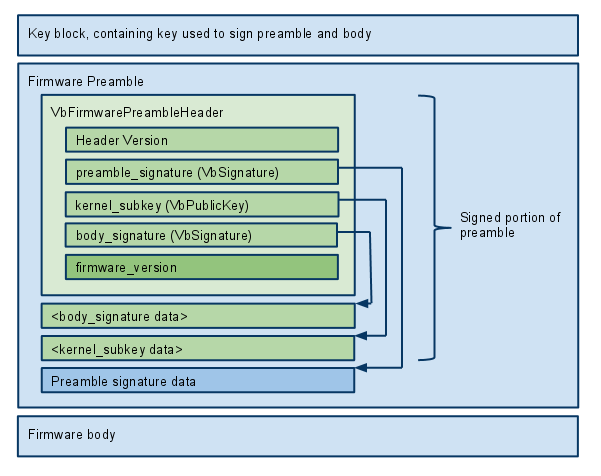
\includegraphics[width=1.0\linewidth]{fw_image.png}
\end{subfigure}%
\begin{subfigure}{.5\textwidth}
  \centering
  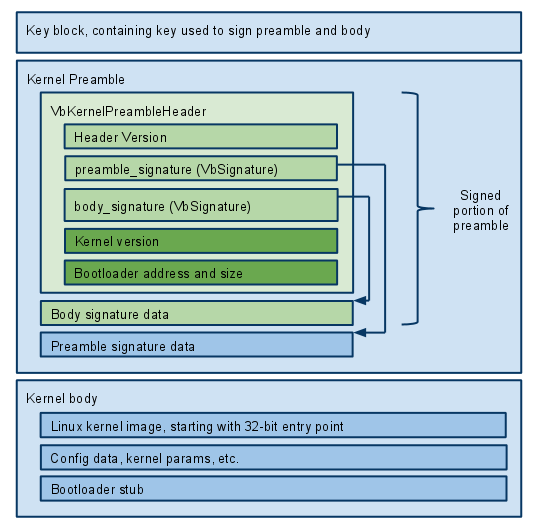
\includegraphics[width=1.0\linewidth]{kernel_image.png}
\end{subfigure}
\caption{Layout of the Firmware and Kernel Images}
\label{fig:vboot_images}
\end{figure}

The actual image is not a data structure but a chunk of data that is stored contiguously in non-volitile memory.
The image structure, as seen in Figure~\ref{fig:vboot_images}, consists of three parts: a key block, a preamble, and the main body of the image.
These parts are accessed in order.
The key block contains a public key that verifies the signature of the preamble and the main body. 
The preamble contains a hash of the image's body which is used to further verify the image's correctness.

The only differences between the two images is in the Preambles.
The Firmware Preamble contains the key that will be used to verify the signature of the Kernel's keyblock.
The Kernel Preamble contains information about the bootloader's address and size instead.

\subsubsection{Key Blocks}

\begin{figure}
\begin{subfigure}{.5\textwidth}
  \centering
  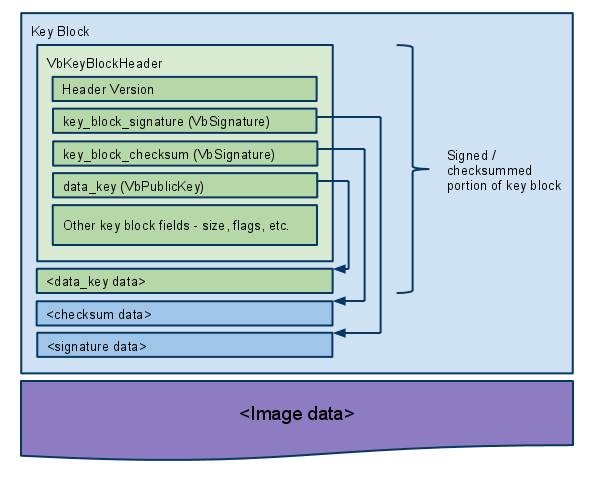
\includegraphics[width=1.0\linewidth]{vboot_keyblock.png}
\end{subfigure}
\begin{subfigure}{.20\textwidth}
  \centering
  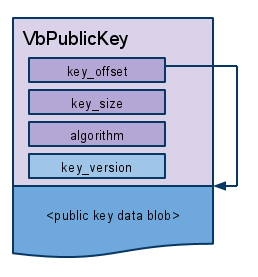
\includegraphics[width=1.0\linewidth]{vbpublickey.png}
\end{subfigure}
\begin{subfigure}{.20\textwidth}
  \centering
  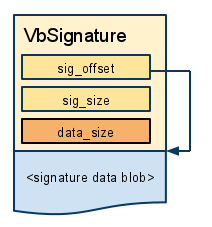
\includegraphics[width=1.0\linewidth]{vbsignature.png}
\end{subfigure}
\caption{The Keyblock data structure and Metadata for Keys and Signatures}
\label{fig:vboot_keyblock}
\end{figure}

The Key block is the first part of the image that is validated and it is used to validate the rest of the image.
The Key block is the data structure that allows a hierarchy of RSA keys to be used during Vboot.
Figure~\ref{fig:vboot_keyblock} shows the structure of the keyblock. 
The key block flags that are mentioned are used to determine which mode of Vboot the Keyblock is valid in. 
There are 4 possible boot modes corresponding to the combination of the two binary options, Developer and Recovery.
% info located in vboot_struct.h

Within the keyblock there exists data structures for a public key and a signature.
Google has added the ability to change their encryption strength.
They have added support for RSA 1024, 2048, 4096, 8192 and for SHA 1, 256, 512, for a total of 12 different possible algorithm combinations.

\subsubsection{Google Binary Block}

% info found in gbb_header.h
The Google Binary Block (GBB) is a part of Vboot's Root of Trust.
It is a data structure stored in Read-Only memory that is initialized and configured in the factory at the laptop's creation.
It contains the Root and Recovery RSA keys, the Hardware ID (HWID) used to identify the specific laptop make and model, a host of flags that affect boot operation, and the bitmaps used for various boot screens.

\end{document}
